\section{最优解的存在}
\label{sec:opt-existence}

$e^x$的例子说明，最优值有限并不保证有点取得它。于是要问：在什么条件下，可以不解问题就断定最优解存在？这个问题值得先回答。若解根本不存在，算法再怎么迭代也找不到它，“收敛”二字也就无从谈起。

\paragraph{从越来越好的候选出发}
设$\bm{C}$非空。按下确界的定义，总能取到一列可行点，使目标值趋于$f^\star$。若$f^\star$有限，就对每个$k$取可行点$\bm{x}^{(k)}$，使$f(\bm{x}^{(k)})\leq f^\star+1/k$；若$f^\star=-\infty$，就取$f(\bm{x}^{(k)})\leq-k$。这样的序列称为\term{最小化序列}（minimizing sequence）。上标$(k)$只是序列编号，这里还没有任何算法。

最小化序列的目标值越来越接近最优值，但序列本身可能乱跑。要从它得到一个最优解，需要依次通过三关：

\begin{enumerate}
 \item 序列留得住：存在收敛的子列，候选不会四散或逃向无穷远；
 \item 极限合法：子列的极限仍然是可行点；
 \item 比较能传到极限：极限处的目标值不高于序列目标值的极限。
\end{enumerate}

前两关由可行集负责，第三关由目标函数负责。图~\ref{fig:opt-existence-failures}中的三个例子各拆掉一关，绿点是最小化序列。

\begin{BookInlineFigure}
  \centering
  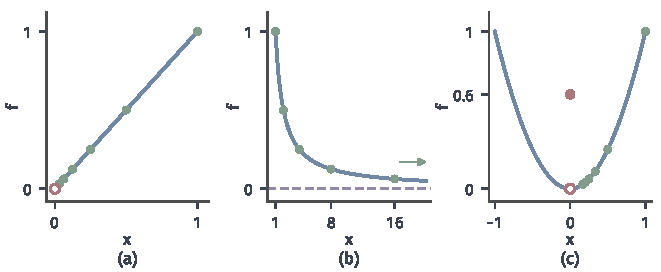
\includegraphics[width=112mm]{figures/05-optimization/01-linear-programming/matplotlib/opt-existence-failures/figure.pdf}
  \caption{存在性论证的三关分别失败。绿点是最小化序列。(a)$f(x)=x$，$C=(0,1]$：序列$2^{-k}$趋于不可行的端点$0$（红色空心点）。(b)$f(x)=1/x$，$C=[1,\infty)$：序列$2^k$逃向无穷远，目标值趋于紫色虚线$0$。(c)$f(x)=x^2$（$x\neq0$），$f(0)=0.6$，$C=[-1,1]$：序列$1/k$趋于$0$，目标值趋于$0$，而$f(0)$跳高到红点$0.6$，值$0$无人取得。}
  \label{fig:opt-existence-failures}
\end{BookInlineFigure}

(a)中$C=(0,1]$有界但不闭，序列有极限$0$，极限却被排除在外，第二关失败。(b)中$C=[1,\infty)$闭但无界，序列$2^k$没有收敛子列，第一关失败。(c)中$C=[-1,1]$很好，序列也收敛到可行点$0$，但函数在$0$处向上跳，极限处的值$0.6$高于序列目标值的极限$0$，第三关失败。

\paragraph{第一关与第二关：紧性}
在$\mathbb{R}^n$中，有界闭集的每个序列都有收敛子列，而且子列的极限仍在集合内。这样的集合称为\term{紧集}（compact set）。紧性恰好一次通过前两关：有界让序列留得住，闭让极限合法。有界闭集的这一性质及一般度量空间中的紧致性，可参考\BookChapterRef{chap:metric-spaces}{卷四第2章“度量空间”}。

\paragraph{第三关：只需要单向的比较}
第三关若用连续性通过，得到的是熟悉的结论：有界闭集上的连续函数取得最小值。仔细看却会发现，连续性要求多了。我们只需要极限处的值“不比序列高”，不需要它“等于序列的极限”。函数在极限点向下跳，只会让极限点更好；不能允许的是向上跳。

\begin{definition}[下半连续]
\label{def:opt-lsc}
设$\bm{C}\subseteq\mathbb{R}^n$，$f:\bm{C}\to\mathbb{R}\cup\{+\infty\}$。若对$\bm{C}$中每个收敛到$\bm{x}\in\bm{C}$的序列$\bm{x}^{(k)}$，都有
\begin{equation}
 f(\bm{x})\leq\liminf_{k\to\infty}f(\bm{x}^{(k)}),
 \label{eq:opt-lsc}
\end{equation}
就称$f$在$\bm{C}$上\term{下半连续}（lower semicontinuous）。
\end{definition}

连续函数满足这个条件且取等号。下半连续还可以用“高度不超过某个水平的部分”来刻画。对实数$a$，称
\begin{equation}
 \bm{S}_a=\{\bm{x}\in\bm{C}:f(\bm{x})\leq a\}
 \label{eq:opt-sublevel}
\end{equation}
为$f$的\term{下水平集}（sublevel set），也就是地形图上高度不超过$a$的区域。

图~\ref{fig:opt-lsc-sublevel}比较两个只在$x=0$一点取值不同的函数。左边$f(0)=0.4$，取跳跃下方的值，下半连续，高度不超过$0.6$的点组成闭区间$[0,0.4]$。右边$f(0)=1$，取跳跃上方的值，不下半连续，同一个下水平集是$(0,0.4]$，缺了左端点。右边的函数沿$x\downarrow0$可以无限接近$0.4$，却被$x=0$处的跳高挡住，最小值取不到。

\begin{BookInlineFigure}
  \centering
  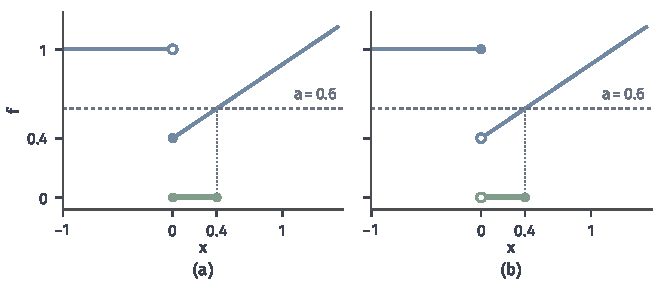
\includegraphics[width=112mm]{figures/05-optimization/01-linear-programming/matplotlib/opt-lsc-sublevel/figure.pdf}
  \caption{下半连续与下水平集的缺口。两个函数在$x<0$时都等于$1$，在$x>0$时都等于$0.4+0.5x$，实心蓝点是$x=0$处的函数值。灰色点线是水平$a=0.6$，绿色线段是下水平集$\bm{S}_{0.6}$。(a)$f(0)=0.4$，下半连续，下水平集是闭区间$[0,0.4]$。(b)$f(0)=1$，向上跳，下水平集$(0,0.4]$缺少左端点。}
  \label{fig:opt-lsc-sublevel}
\end{BookInlineFigure}

图中的观察就是下面的引理：下半连续性的作用，是让下水平集不缺边界。

\begin{lemma}[下半连续与闭下水平集]
\label{lem:opt-lsc-sublevel}
设$\bm{C}\subseteq\mathbb{R}^n$是闭集，$f:\bm{C}\to\mathbb{R}\cup\{+\infty\}$。$f$在$\bm{C}$上下半连续，当且仅当对每个$a\in\mathbb{R}$，下水平集$\bm{S}_a$是闭集。
\end{lemma}

\begin{proof}
先设$f$下半连续。取$\bm{S}_a$中的序列$\bm{x}^{(k)}$，设它收敛到$\bm{x}$。$\bm{C}$是闭集，所以$\bm{x}\in\bm{C}$。由下半连续性，
\[
 f(\bm{x})\leq\liminf_{k\to\infty}f(\bm{x}^{(k)})\leq a.
\]
所以$\bm{x}\in\bm{S}_a$，$\bm{S}_a$是闭集。

反过来，设每个$\bm{S}_a$都是闭集，但$f$在某点$\bm{x}\in\bm{C}$不满足式~\eqref{eq:opt-lsc}，即存在$\bm{C}$中收敛到$\bm{x}$的序列，使$\liminf_kf(\bm{x}^{(k)})<f(\bm{x})$。取实数$a$严格介于这两个量之间。下极限小于$a$，所以有子列$\bm{x}^{(k_j)}$始终满足$f(\bm{x}^{(k_j)})\leq a$，也就是子列落在$\bm{S}_a$中。

$\bm{S}_a$是闭集，子列的极限$\bm{x}$也在其中，于是$f(\bm{x})\leq a$。这与$a<f(\bm{x})$矛盾。
\end{proof}

\paragraph{紧可行集上的存在定理}
三关齐备，就得到第一个存在定理。

\begin{theorem}[紧可行集上的最小值]
\label{thm:opt-compact-existence}
设$\bm{C}\subseteq\mathbb{R}^n$非空且紧，$f:\bm{C}\to\mathbb{R}\cup\{+\infty\}$在$\bm{C}$上下半连续，且至少有一点取有限值。则最优值$f^\star$是有限实数，且最优解存在。
\end{theorem}

\begin{proof}
由假设，$f^\star<+\infty$。取一个最小化序列$\bm{x}^{(k)}\in\bm{C}$。$\bm{C}$是紧集，所以有子列$\bm{x}^{(k_j)}$收敛到某个$\bm{x}^\star\in\bm{C}$。由下半连续性，
\[
 f(\bm{x}^\star)\leq\liminf_{j\to\infty}f(\bm{x}^{(k_j)})=f^\star.
\]

若$f^\star=-\infty$，上式给出$f(\bm{x}^\star)=-\infty$，与$f$不取$-\infty$矛盾，所以$f^\star$有限。又因$\bm{x}^\star$可行，有$f(\bm{x}^\star)\geq f^\star$。两个不等式合起来得到
\[
 f(\bm{x}^\star)=f^\star.
\]
所以$\bm{x}^\star$是最优解。
\end{proof}

资源分配的可行集由四个闭半平面相交而成，它有界且闭，目标是线性函数，因而连续。定理~\ref{thm:opt-compact-existence}立刻保证最优解存在。这个结论不需要知道解在$(2,2)$，它只告诉我们值得去找。

定理的条件都是充分条件。例如$f(x)=x^2$的可行集$\mathbb{R}$无界，最小点$x=0$依然存在。图~\ref{fig:opt-existence-failures}的三个例子说明的是：逐条去掉条件后，结论可能不成立。

\paragraph{无界可行集：只看不太差的点}
二次拟合的可行集是整个$\mathbb{R}^n$，它不紧，定理~\ref{thm:opt-compact-existence}不能直接用。但我们并不需要整个可行集紧，只需要把最小化序列关进某个紧集。取一个有限的水平$a$，使下水平集$\bm{S}_a$非空。凡是目标值高于$a$的点都比$\bm{S}_a$中的点差，不可能是最优解，可以直接丢掉。剩下要看的只有$\bm{S}_a$。

\begin{theorem}[紧下水平集保证存在]
\label{thm:opt-compact-sublevel}
设$f:\bm{C}\to\mathbb{R}\cup\{+\infty\}$在$\bm{C}$上下半连续。若存在实数$a$，使下水平集$\bm{S}_a$非空且紧，则$f^\star$是有限实数，且最优解存在。
\end{theorem}

\begin{proof}
$f$限制在紧集$\bm{S}_a$上仍下半连续，并在$\bm{S}_a$上取有限值。由定理~\ref{thm:opt-compact-existence}，存在$\bm{x}^\star\in\bm{S}_a$，使$f(\bm{x}^\star)=\min_{\bm{S}_a}f\leq a$。

对$\bm{C}\setminus\bm{S}_a$中的点，有$f(\bm{x})>a\geq f(\bm{x}^\star)$。所以$\bm{x}^\star$是$f$在整个$\bm{C}$上的最小点，$f^\star=f(\bm{x}^\star)$有限。
\end{proof}

这个定理只要求有一个下水平集紧，其余的下水平集可以无界。在$\mathbb{R}$上考虑
\[
 f(x)=\frac{x^2}{1+x^2}.
\]
令$a=1/2$，解不等式$f(x)\leq1/2$，得到$x^2\leq1$，所以$\bm{S}_{1/2}=[-1,1]$是紧集，最小点$x=0$由此得到保证。而取$a\geq1$时，下水平集是整个$\mathbb{R}$，无界。

怎样检验下水平集紧？闭性由引理~\ref{lem:opt-lsc-sublevel}给出，只要$\bm{C}$闭、$f$下半连续。有界性则需要目标在远处足够高，这就是强制性。

\begin{definition}[强制性]
\label{def:opt-coercive}
设$\bm{C}\subseteq\mathbb{R}^n$，$f:\bm{C}\to\mathbb{R}\cup\{+\infty\}$。若对$\bm{C}$中任意满足$\lVert\bm{x}^{(k)}\rVert_2\to\infty$的序列，都有$f(\bm{x}^{(k)})\to+\infty$，就称$f$在$\bm{C}$上是\term{强制的}（coercive）。
\end{definition}

强制性等价于每个下水平集都有界。若某个$\bm{S}_a$无界，从中取范数趋于无穷的序列，其目标值始终不超过$a$，不满足强制性。反过来，若各下水平集都有界，而$\lVert\bm{x}^{(k)}\rVert_2\to\infty$，则对任意$a$，序列最终离开$\bm{S}_a$，也就是最终$f(\bm{x}^{(k)})>a$，所以$f(\bm{x}^{(k)})\to+\infty$。

于是得到实际最常用的形式：若$\bm{C}$非空闭，$f$下半连续且强制，并在$\bm{C}$上至少有一点取有限值，则最优解存在。这只需取$a$为该点的函数值，再用定理~\ref{thm:opt-compact-sublevel}。各条件的分工是：强制性使下水平集有界，留住了序列；$\bm{C}$闭与下半连续使下水平集闭，留住了极限。

\paragraph{回到二次拟合}
对式~\eqref{eq:opt-ridge}逐项核对。$f$是多项式，处处有限且连续；$\bm{C}=\mathbb{R}^n$是闭集。当$\gamma>0$时，拟合项非负，所以
\[
 f(\bm{x})\geq\frac{\gamma}{2}\lVert\bm{x}\rVert_2^2.
\]
范数趋于无穷时目标趋于无穷，$f$强制，最优解存在。

$\gamma=0$时情况不同。对实例~\eqref{eq:opt-ridge-instance}，沿方向$(1,-1)$目标不变：取$\bm{x}^{(k)}=(1+k,1-k)$，范数趋于无穷而$f=0$，所以$f$不强制。图~\ref{fig:opt-coercive-sublevel}比较了两种情形，同一个水平$a=1$的下水平集，在$\gamma=0$时是无界的带，在$\gamma=0.5$时收缩成一个椭圆。

\begin{BookInlineFigure}
  \centering
  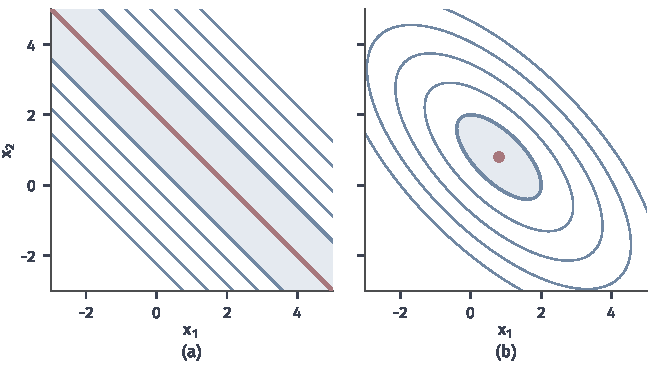
\includegraphics[width=112mm]{figures/05-optimization/01-linear-programming/matplotlib/opt-coercive-sublevel/figure.pdf}
  \caption{二次拟合实例$f(\bm{x})=\frac12(x_1+x_2-2)^2+\frac{\gamma}{2}\lVert\bm{x}\rVert_2^2$的下水平集。浅蓝区域及其粗边界是$\{f\leq1\}$，细线是其他等高线。(a)$\gamma=0$：下水平集是两条平行线之间的无界带，红线$x_1+x_2=2$是最优解集合。(b)$\gamma=0.5$：下水平集是椭圆，红点是唯一最优解$(0.8,0.8)$。}
  \label{fig:opt-coercive-sublevel}
\end{BookInlineFigure}

然而$\gamma=0$时最优解仍然存在，整条直线$x_1+x_2=2$都是。这再次说明强制性只是充分条件。对一般的$\bm{A}$，不带正则项的最小二乘总有解，依据是正规方程$\bm{A}^\top\bm{A}\bm{x}=\bm{A}^\top\bm{b}$总可解，可参考\BookChapterRef{chap:linear-solution-selection}{卷二第11章“线性方程与最小二乘的选解”}，这里用不到强制性。

\paragraph{有限维的边界}
整个论证依赖“有界闭集紧”，这是有限维空间的性质。平方可和的数列空间中，第$k$个坐标为$1$、其余为$0$的数列组成一列单位向量，它们两两距离都是$\sqrt2$，都在闭单位球里，却没有收敛子列。函数空间上的存在性要换一种收敛概念，第~\ref{chap:functional-optimization-variation}章会处理这件事；在$\mathbb{R}^n$中，本节的定理已经够用。
